\documentclass[aspectratio=169]{beamer}

\mode<presentation>
{
  \usetheme{Frankfurt}
  \usecolortheme{crane}
  \usefonttheme{default}
  \setbeamertemplate{navigation symbols}{}
  \setbeamertemplate{caption}[numbered]
}

\usepackage[english]{babel}
\usepackage[T1]{fontenc}
\usepackage[utf8]{inputenc}
\usepackage{booktabs}
\usepackage{amsmath}
\usepackage{array}
\usepackage{graphicx}

\graphicspath{{../reports/figures/}}

\title[Traffic Speed Forecasting on PEMS08]
{Forecasting Average Traffic Speed\\on the PEMS08 Sensor Network}
\subtitle{Near-future and long-term traffic speed forecasting}
\author[Vita Naglič, Matevž Rom, Nace Kovačič]
{Vita Naglič \and Matevž Rom \and Nace Kovačič}
\institute{Artificial Intelligence}
\date{}

\setbeamertemplate{footline}
{
  \leavevmode%
  \hbox{%
  \begin{beamercolorbox}[wd=.42\paperwidth,ht=2.4ex,dp=1.1ex,center]{author in head/foot}%
    \usebeamerfont{author in head/foot}\insertshortauthor{} (Artificial Intelligence)
  \end{beamercolorbox}%
  \begin{beamercolorbox}[wd=.43\paperwidth,ht=2.4ex,dp=1.1ex,center]{title in head/foot}%
    \usebeamerfont{title in head/foot}\insertshorttitle
  \end{beamercolorbox}%
  \begin{beamercolorbox}[wd=.15\paperwidth,ht=2.4ex,dp=1.1ex,center]{date in head/foot}%
    \usebeamerfont{date in head/foot}\insertframenumber{} / \inserttotalframenumber
  \end{beamercolorbox}}%
  \vskip0pt%
}

\newcommand{\missingfigure}[2]{%
  \begin{center}
    \fbox{%
      \begin{minipage}[c][#1][c]{0.88\linewidth}
        \centering
        \textbf{Placeholder}\\[0.5em]
        #2
      \end{minipage}
    }
  \end{center}
}

\begin{document}

\begin{frame}
  \titlepage
\end{frame}

\section{Introduction}

\begin{frame}{Traffic Speed Forecasting as Graph Time Series}
\fontsize{8}{9.6}\selectfont
\begin{columns}[T,totalwidth=\textwidth]
\begin{column}{0.36\textwidth}
\textbf{Task}

Recent sensor history $\rightarrow$ future sensor speed?

\vspace{0.6em}
\textbf{Forecast ranges}

\begin{itemize}
  \item near future: +5 to +60 min
  \item longer term: +1h, +3h, +6h, +12h
\end{itemize}

\vspace{0.6em}
\textbf{Graph view}

\begin{itemize}
  \item node-level regression
  \item sensor time series
  \item neighbour traffic context
\end{itemize}

\vspace{0.4em}
\textbf{Use case:} travel time, congestion warnings, routing
\end{column}
\begin{column}{0.61\textwidth}
\centering
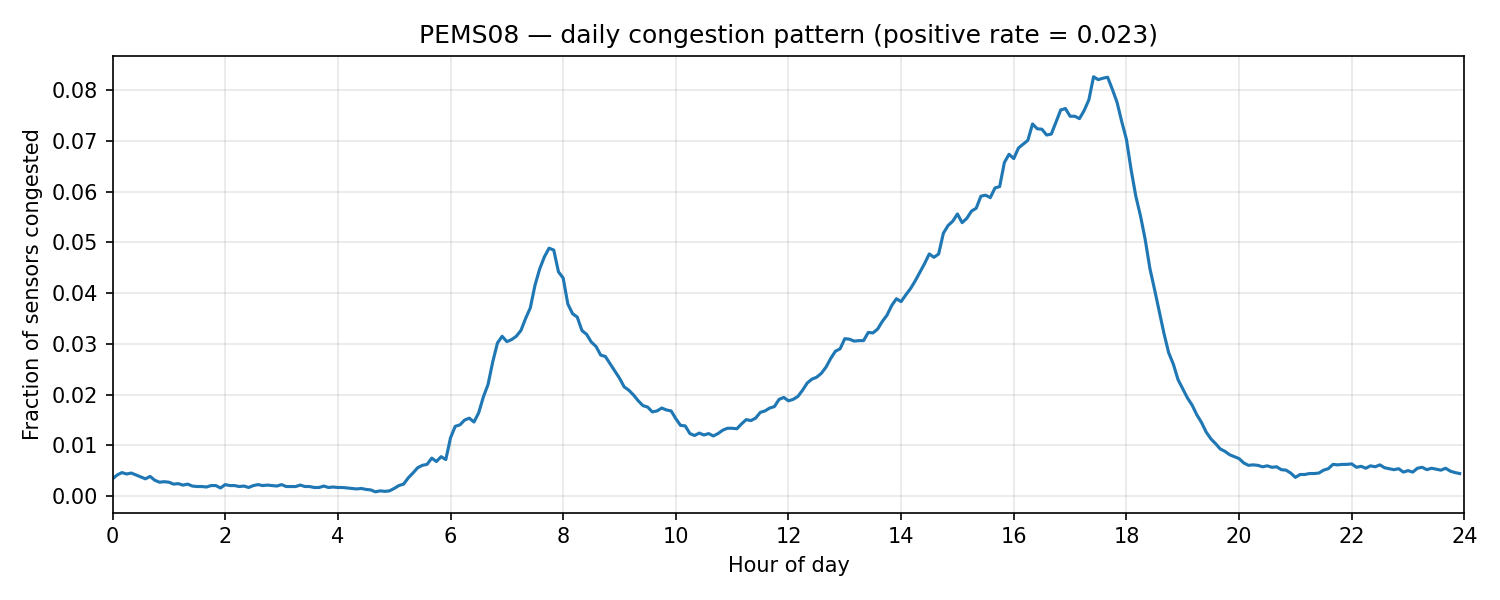
\includegraphics[width=\linewidth,height=0.66\textheight,keepaspectratio]{pems08_daily_congestion.png}
\vspace{-0.9em}

Daily congestion pattern; positive rate: 2.27\%.
\end{column}
\end{columns}
\end{frame}

\section{Dataset}

\begin{frame}{PEMS08: Sparse, Connected Road Graph}
\footnotesize
\begin{columns}[T,totalwidth=\textwidth]
\begin{column}{0.55\textwidth}
\begin{figure}
  \centering
  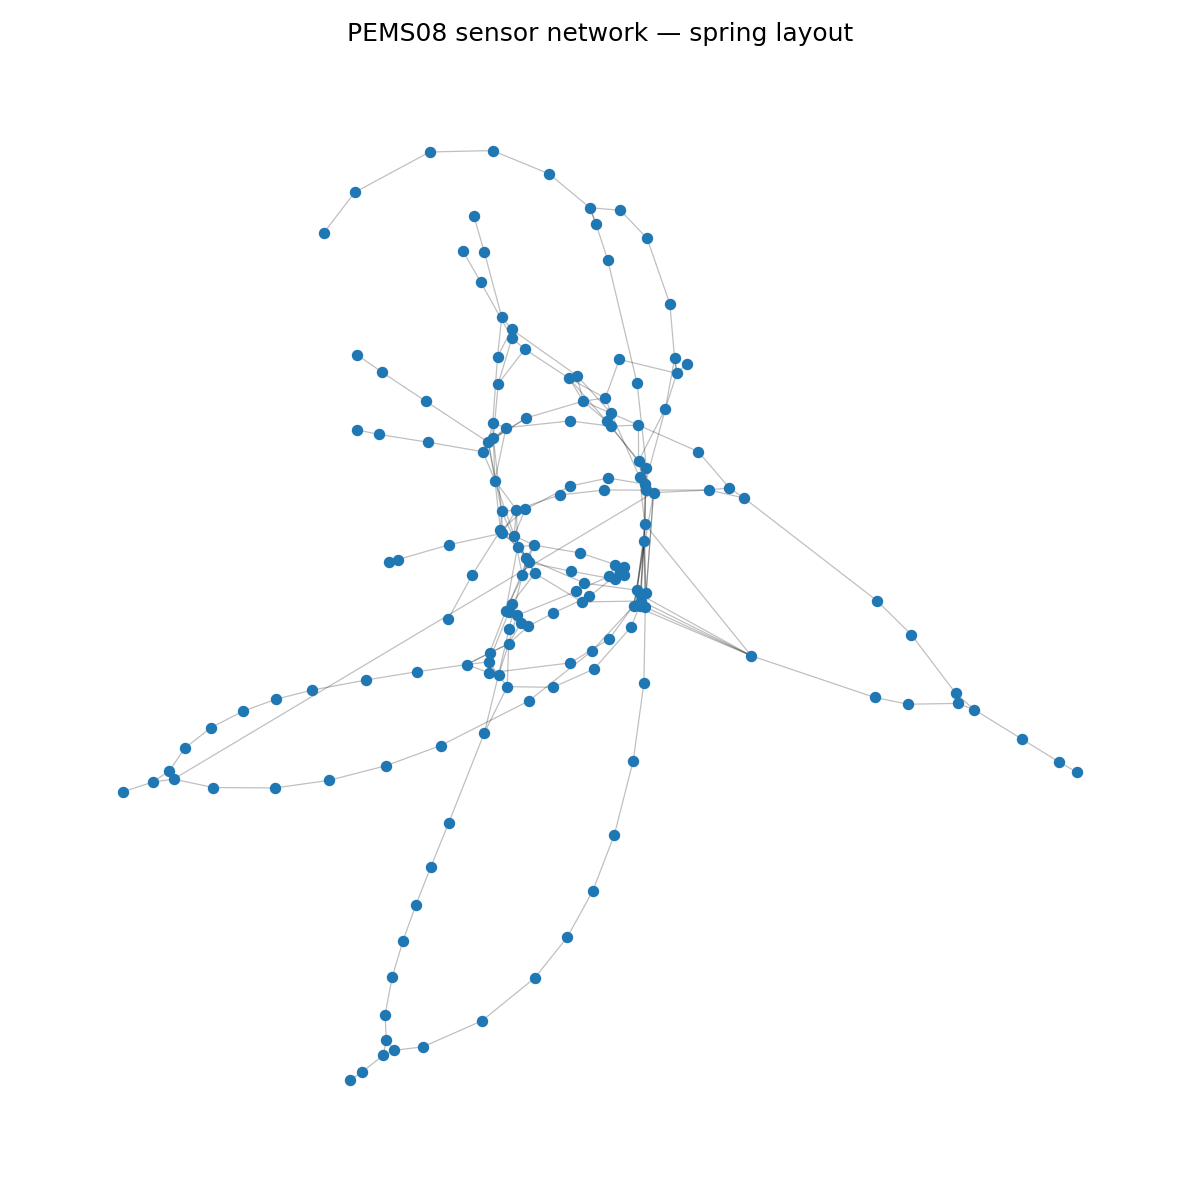
\includegraphics[width=\linewidth,height=0.8\textheight,keepaspectratio]{pems08_network_layout.png}
\end{figure}
\end{column}
\begin{column}{0.40\textwidth}
\textbf{PEMS08 benchmark}

\vspace{0.3em}
\begin{tabular}{@{}ll@{}}
\toprule
sensors & \textbf{170} \\
time steps & \textbf{17,856} \\
resolution & \textbf{5 min} \\
duration & \textbf{62 days} \\
\bottomrule
\end{tabular}

\vspace{0.7em}
\textbf{Road graph facts}
\begin{itemize}
  \item 277 unique directed edges
  \item 1 weakly connected component
  \item avg in/out-degree: 1.63
  \item 16 Louvain communities
\end{itemize}

\vspace{0.5em}
\textbf{Modeling consequence}

Sensor history + nearby-road context
\end{column}
\end{columns}
\end{frame}

\section[NN1]{Neural Network 1: 60 minutes ahead}

\begin{frame}{NN1: 60-Minute Speed Forecast}
\small
\textbf{Task}
\begin{itemize}
  \item one speed value per sensor
  \item horizon: +60 min
  \item input window: previous 12 readings = 1 hour
\end{itemize}

\vspace{0.7em}
\textbf{Features per sensor and time step}
\begin{itemize}
  \item flow, occupancy, speed
  \item time-of-day and day-of-week
  \item incoming-neighbour averages
\end{itemize}

\vspace{0.7em}
\textbf{Input/output shape}

\[
[12, 170, 10] \rightarrow [170]
\]
\end{frame}

\begin{frame}{NN1/NN2: Split and Leakage Control}
\small
\textbf{Chronological split}

\begin{itemize}
  \item train / validation / test = 60\% / 20\% / 20\%
  \item train = past, test = future
  \item no random k-fold on autocorrelated time series
\end{itemize}

\vspace{0.7em}
\textbf{Normalisation}

\begin{itemize}
  \item per-sensor z-score
  \item training statistics only
  \item metrics after denormalising to mph
\end{itemize}

\vspace{0.7em}
\textbf{Boundary gap}

\[
W = 12 \text{ steps}
\]

Input windows never cross split boundaries.
\end{frame}

\begin{frame}{NN1/NN2: GCN-GRU Architecture}
\footnotesize
\textbf{Spatial step}
\[
H = \operatorname{ReLU}(A X W_{\mathrm{gcn}}), \qquad
A = \alpha A_{\mathrm{fixed}} + (1-\alpha)\tilde{A}, \qquad
\tilde{A} = \operatorname{softmax}(\operatorname{ReLU}(E_1E_2^\top)).
\]

\vspace{-0.4em}
\begin{columns}[T,totalwidth=\textwidth]
\begin{column}{0.48\textwidth}
\textbf{Architecture}
\begin{itemize}
  \item 2 graph-convolution layers
  \item adaptive adjacency
  \item residual node signal
  \item 2-layer GRU over 12 steps
\end{itemize}
\end{column}
\begin{column}{0.47\textwidth}
\textbf{Training}
\begin{itemize}
  \item Huber loss, $\delta = 1$
  \item Adam, lr $10^{-3}$
  \item early stopping on validation MAE
  \item seed 42
\end{itemize}
\end{column}
\end{columns}
\end{frame}

\section[NN2]{Neural Network 2: interval [+5, +60] minutes}

\begin{frame}{NN2: Full +5 to +60 Minute Curve}
\small
\textbf{Task}

\begin{itemize}
  \item speed at 5, 10, \ldots, 60 min
  \item one value per sensor and horizon
  \item same input window and features as NN1
  \item standard multi-horizon benchmark setup
\end{itemize}

\vspace{0.8em}
\textbf{Input/output shape}

\[
[12, 170, 10] \rightarrow [170, 12]
\]

\vspace{0.5em}
\texttt{--single-horizon} selects NN1; default mode trains NN2.
\end{frame}

\begin{frame}{NN2: One Head Predicts All Horizons}
\small
\textbf{Same core model}
\begin{itemize}
  \item spatial GCN
  \item adaptive adjacency + residual
  \item temporal GRU
  \item same split and normalisation
\end{itemize}

\vspace{0.8em}
\textbf{Only the output head changes}
\[
\operatorname{Linear}(\mathrm{hidden} \to 1)
\quad \Longrightarrow \quad
\operatorname{Linear}(\mathrm{hidden} \to 12)
\]

\vspace{0.7em}
\textbf{Best run}
\begin{itemize}
  \item NN1: 58,954 parameters
  \item NN2: 59,669 parameters
  \item extra output horizons with almost no parameter cost
\end{itemize}
\end{frame}

\section[NN3]{Neural Network 3: long-term horizons}

\begin{frame}{NN3: Later-Today Speed Forecasting}
\footnotesize
\textbf{Goal:} from immediate traffic control to later-today planning

\vspace{0.5em}
\begin{columns}[T,totalwidth=\textwidth]
\begin{column}{0.48\textwidth}
\textbf{Prediction horizons}

\vspace{0.3em}
\begin{center}
\renewcommand{\arraystretch}{1.25}
\begin{tabular}{@{}cccc@{}}
\toprule
\textbf{+1h} & \textbf{+3h} & \textbf{+6h} & \textbf{+12h} \\
12 steps & 36 steps & 72 steps & 144 steps \\
\bottomrule
\end{tabular}
\end{center}

\vspace{0.5em}
\textbf{Target}

\begin{itemize}
  \item speed per sensor
  \item 4 horizons jointly
\end{itemize}
\end{column}
\begin{column}{0.47\textwidth}
\textbf{Leakage-safe inputs}
\begin{itemize}
  \item flow, occupancy, speed at $t$
  \item speed lags: 3h, 6h, 12h, 1d, 2d, 7d
  \item current + target calendar time
\end{itemize}

\vspace{0.4em}
\textbf{Built dataset}
\begin{tabular}{@{}ll@{}}
$X$ & $(15696, 170, 29)$ \\
$y$ & $(15696, 170, 4)$ \\
train / val / test & 9417 / 3139 / 3140 \\
\end{tabular}
\end{column}
\end{columns}

\vspace{0.35em}
\centering
\textbf{No future traffic measurements as inputs}
\end{frame}

\begin{frame}{NN3: Shared-Sensor GRU}
\small
\begin{center}
\large
2 hours of features $\rightarrow$ shared GRU $\rightarrow$ +1h, +3h, +6h, +12h speeds
\end{center}

\vspace{0.4em}
\begin{columns}[T,totalwidth=\textwidth]
\begin{column}{0.48\textwidth}
\textbf{Why this architecture}
\begin{itemize}
  \item small, stable model
  \item temporal patterns shared across sensors
  \item all long horizons in one pass
\end{itemize}
\end{column}
\begin{column}{0.47\textwidth}
\textbf{Best run}
\begin{itemize}
  \item input window: 24 steps = 2 hours
  \item hidden size: 64
  \item GRU layers: 2
  \item dropout: 0.2
  \item parameters: 43,460
  \item loss: Smooth L1 / Huber
\end{itemize}
\end{column}
\end{columns}

\vspace{0.6em}
\centering
\textbf{Train-only normalisation; metrics in mph}
\end{frame}

\section{Results}

\begin{frame}{Results: NN1 vs NN2 vs Persistence}
\small
\begin{center}
\renewcommand{\arraystretch}{1.18}
\setlength{\tabcolsep}{0.85em}
\begin{tabular}{@{}lccc@{}}
\toprule
Model (test set) & MAE & RMSE & MAPE \\
\midrule
Persistence (avg over 5--60 min) & 1.6133 & 3.7811 & 3.08\% \\
Persistence (60 min only) & 2.1403 & 4.9692 & 4.21\% \\
\addlinespace
NN1 -- single-horizon (60 min) & 1.7979 & 4.4583 & 4.13\% \\
NN2 -- multi-horizon (60 min) & \textbf{1.7677} & 4.2927 & 3.98\% \\
NN2 -- multi-horizon (avg) & \textbf{1.4897} & 3.6037 & 3.23\% \\
\bottomrule
\end{tabular}
\end{center}

\vspace{0.7em}
\begin{itemize}
  \item 60 min: NN2 1.7677 vs. NN1 1.7979 MAE.
  \item 60-min persistence improvement: 17.4\%.
  \item average persistence improvement: 7.7\%.
\end{itemize}
\end{frame}

\begin{frame}{Results: Per-Horizon Crossover}
\small
\begin{columns}[T,totalwidth=\textwidth]
\begin{column}{0.62\textwidth}
\includegraphics[width=\linewidth,height=0.67\textheight,keepaspectratio]{pems08_results_crossover.png}
\end{column}
\begin{column}{0.33\textwidth}
\textbf{Pattern}

\begin{itemize}
  \item 5--15 min: persistence wins
  \item $\sim$20 min: crossover
  \item 60 min: NN2 wins by 0.3726 MAE
\end{itemize}

\vspace{0.5em}
\textbf{Reason}

Short-term speed changes slowly; longer horizons need learned temporal-spatial patterns.
\end{column}
\end{columns}
\end{frame}

\begin{frame}{Results: Architecture Ablation}
\small
\begin{columns}[T,totalwidth=\textwidth]
\begin{column}{0.62\textwidth}
\includegraphics[width=\linewidth,height=0.67\textheight,keepaspectratio]{pems08_results_ablation.png}
\end{column}
\begin{column}{0.33\textwidth}
\textbf{Pattern}

\begin{itemize}
  \item fixed graph: weakest
  \item + adaptive: lower MAE
  \item + residual: lower MAE again
\end{itemize}

\vspace{0.4em}
\textbf{Takeaway}

Architecture gains, not only model scale.
\end{column}
\end{columns}
\end{frame}

\begin{frame}{Results: NN3 Long-Horizon Forecasts}
\footnotesize
\begin{columns}[T,totalwidth=\textwidth]
\begin{column}{0.60\textwidth}
  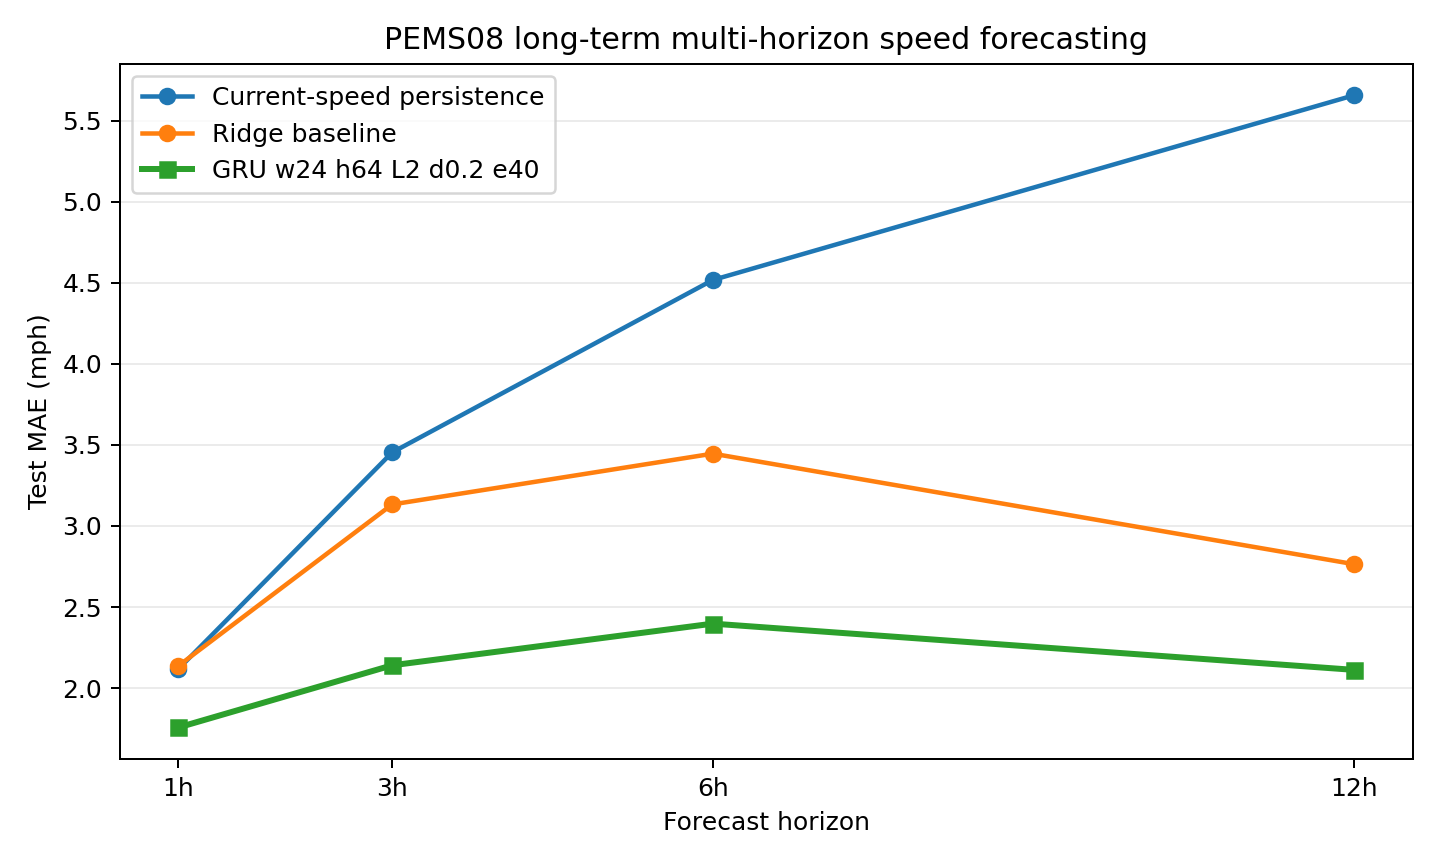
\includegraphics[width=\linewidth,height=0.60\textheight,keepaspectratio]{pems08_longterm_multi_horizon_mae.png}
\end{column}
\begin{column}{0.38\textwidth}
\centering
\scriptsize
\renewcommand{\arraystretch}{1.18}
\setlength{\tabcolsep}{0.45em}
\begin{tabular}{@{}lrr@{}}
\toprule
Metric & Ridge & GRU \\
\midrule
Avg MAE & 2.8699 & 2.1015 \\
+1h MAE & 2.1364 & 1.7566 \\
+3h MAE & 3.1328 & 2.1402 \\
+6h MAE & 3.4462 & 2.3974 \\
+12h MAE & 2.7640 & 2.1120 \\
\bottomrule
\end{tabular}
\end{column}
\end{columns}
\end{frame}

\begin{frame}{Takeaways}
\large
\begin{itemize}
  \item PEMS08: graph time-series forecasting
  \item short horizons: immediate traffic dynamics
  \item NN3: later-today horizons (+1h, +3h, +6h, +12h)
  \item chronological splits + leakage checks
  \item best long-horizon GRU: lowest MAE at every horizon
\end{itemize}
\end{frame}

\end{document}
